\documentclass[12pt]{scrreprt}%{article} % Beginn der LaTeX-Datei
\usepackage{amsmath,amssymb}  % erleichtert Mathe 
\usepackage{MnSymbol}
\usepackage{wasysym}
\usepackage[arrow,matrix,curve]{xy}  % Für kommutative Homomorphismen-Diagramme 

\usepackage{enumerate}   % Für variieren der Nummerierungs-Symbole
\usepackage{hyperref}  % Für klickbare und rot umrandete Labels
\usepackage{bbm}     % Für Einheitsmatrix-Symbol

\usepackage{blindtext}
\usepackage{graphicx} % fuer Grafik-Einbindung
%\usepackage[dvips]{hyperref}
\usepackage{ngerman}
\usepackage[utf8]{inputenc}      % = Umlaute unter Windows 
                                   % Linux = \usepackage[latin1]{inputenc}
                                   % Mac = \usepackage[applemac]{inputenc}
\usepackage{color}
%  ermoeglicht, farbigen Text zu drucken.
% Und nun werden die Farben definiert.
\definecolor{white}{rgb}{1,1,1}
\definecolor{darkred}{rgb}{0.3,0,0}
\definecolor{darkgreen}{rgb}{0,0.3,0}
\definecolor{darkblue}{rgb}{0,0,0.3}
\definecolor{pink}{rgb}{0.78,0.09,0.51}
\definecolor{purple}{rgb}{0.28,0.24,0.55}
\definecolor{orange}{rgb}{1,0.6,0.0}
\definecolor{grey}{rgb}{0.4,0.4,0.4}
\definecolor{aquamarine}{rgb}{0.4,0.8,0.65}


\DeclareMathOperator{\GL}{GL} % einige Macros
\newcommand{\N}{\mathbb{N}}
\newcommand{\Z}{\mathbb{Z}}
\newcommand{\Q}{\mathbb{Q}}
\newcommand{\R}{\mathbb{R}}
\newcommand{\C}{\mathbb{C}}
\newcommand{\K}{\mathbb{K}}
\newcommand{\cP}{{\mathcal P}} 
\newcommand{\qed}{\newline \mbox{~} \hfill$\square$}
\newcommand{\q}{\quad}  % Abstand in normaler Umgebung und in Mathe-Umgebung
\newcommand{\CS}{\mathbb{C}^*}
\newcommand{\RS}{\mathbb{R}^*}
\newcommand{\QS}{\mathbb{Q}^*}
\newcommand{\ZS}{\mathbb{Z}^*}
\newcommand{\KS}{\mathbb{K}^*}
\newcommand{\zl}{\textless} 
\newcommand{\zr}{\textgreater} 
\newcommand{\zM}{\zl M\zr} 
\newcommand{\mat}[4]{\left(\begin{matrix} #1 & #2 \\ #3 & #4\end{matrix}\right)}  % 2x2-Matrix
\newcommand{\vect}[2]{\left(\begin{matrix} #1 \\ #2\end{matrix}\right)}  % 2x2-Matrix
\newcommand{\sdpa}{\rtimes_\alpha} 
\newcommand{\blitz}{\lightning} 
\newcommand{\orbit}{\mathcal{O}} 

%\newcommand{\M}{\text{M}}  %sorgt für kursives M in kursivem Text, wie Definitionen, also ungeeignet.
\DeclareMathOperator{\M}{M}   %besser, macht es immer aufrecht  
\DeclareMathOperator{\SL}{SL} 
\DeclareMathOperator{\Id}{Id}   
\DeclareMathOperator{\Aff}{Aff}  
\DeclareMathOperator{\linear}{linear}  
\DeclareMathOperator{\injektiv}{injektiv}  
\DeclareMathOperator{\surjektiv}{surjektiv} 
\DeclareMathOperator{\bijektiv}{bijektiv}  
\DeclareMathOperator{\und}{und}  
\DeclareMathOperator{\OO}{O}  
\DeclareMathOperator{\SO}{SO}  
\DeclareMathOperator{\U}{U} 
\DeclareMathOperator{\ord}{ord} 
\DeclareMathOperator{\ggT}{ggT} 
\DeclareMathOperator{\kgV}{kgV} 
\DeclareMathOperator{\oee}{\OE} 
\DeclareMathOperator{\im}{im} 
\DeclareMathOperator{\Aut}{Aut} 
\DeclareMathOperator{\ist}{ist} 
\DeclareMathOperator{\Automorphismus}{Automorphismus} 
\DeclareMathOperator{\Hom}{Hom.} 
\DeclareMathOperator{\EM}{\mathbbm{1}} 
\DeclareMathOperator{\fest}{fest} 
\DeclareMathOperator{\sgn}{sgn} 
\DeclareMathOperator{\dv}{\mathbin{\dot{\cup}}}      % disjunkte Vereinigung klein
\DeclareMathOperator{\gdv}{\mathbin{\dot{\bigcup}}}      % disjunkte Vereinigung groß
\DeclareMathOperator{\nt}{\trianglelefteq}           % Normalteiler
\DeclareMathOperator{\nnt}{\ntrianglelefteq}           % Normalteiler
\DeclareMathOperator{\abelsch}{abelsch}     
\DeclareMathOperator{\Lemma}{Lemma}  
\DeclareMathOperator{\Lagrange}{Lagrange}  
\DeclareMathOperator{\assoziativ}{assoziativ}  
\DeclareMathOperator{\varphit}{\tilde{\varphi}}  
\DeclareMathOperator{\Def}{Def.}
\DeclareMathOperator{\ug}{\leq}  
\DeclareMathOperator{\iso}{\simeq} 
\DeclareMathOperator{\NT}{NT} 
\DeclareMathOperator{\UG}{UG} 
\DeclareMathOperator{\da}{\text{ da }} 
\DeclareMathOperator{\Satz}{Satz}  
\DeclareMathOperator{\niso}{\nsimeq} 
\DeclareMathOperator{\hier}{hier} 
\DeclareMathOperator{\IV}{IV} 
\DeclareMathOperator{\oder}{oder} 
\DeclareMathOperator{\Bemerkung}{Bemerkung} 
\DeclareMathOperator{\Mot}{Mot} 
\DeclareMathOperator{\diag}{diag} 
\DeclareMathOperator{\Gruppenwirkung}{Gruppenwirkung} 
\DeclareMathOperator{\sonst}{sonst} 
\DeclareMathOperator{\Fix}{Fix} 
\DeclareMathOperator{\Kreis}{Kreis} 
\DeclareMathOperator{\Iso}{Iso} 

\newtheorem{deff}{Definition}[chapter]
\newtheorem{satz}[deff]{Satz}
%\newtheorem{beweis}{Beweis}         % so wäre Beweis nummeriert
\newtheorem{theorem}[deff]{Theorem}
\newtheorem{lemma}[deff]{Lemma}
\newtheorem{proposition}[deff]{Proposition}
\newtheorem{korollar}[deff]{Korollar}
\newtheorem{bem}[deff]{Bemerkung}
\newtheorem{bsp}[deff]{Beispiel}
\newtheorem{anm}[deff]{Anmerkung}
\newtheorem{folg}[deff]{Folgerung}
%\newtheorem{wdh}[deff]{Wiederholung}         % so wäre Wiederholung nummeriert


\newenvironment{beweis}[1][Beweis]{\begin{trivlist}    % so ist Beweis nicht nummeriert
\item[\hskip \labelsep {\bfseries #1}]}{\end{trivlist}}
\newenvironment{wdh}[1][Wiederholung]{\begin{trivlist}    % so ist Wiederholung nicht nummeriert
\item[\hskip \labelsep {\bfseries #1}]}{\end{trivlist}}
%\newenvironment{bsp}[1][Beispiel]{\begin{trivlist}
%\item[\hskip \labelsep {\bfseries #1}]}{\end{trivlist}}
%\newenvironment{bem}[1][Bemerkung]{\begin{trivlist}
%\item[\hskip \labelsep {\bfseries #1}]}{\end{trivlist}}


\renewcommand{\labelenumi}{(\theenumi)} % Änderung von "1." zu "(1)" in Aufzählungen



% Vorlesungscounter abschalten:
%ersetze "small" durch "tiny"
%ersetze "grey" durch "white"
%ersetze "\rule{1\textwidth}{0.4pt}\newline" durch "~"
\newcommand{\groesse}{\small}
\newcommand{\farbe}{\color{grey}}
\newcommand{\linie}{\rule{1\textwidth}{0.4pt}\newline}
%\newcommand{\groesse}{\tiny}
%\newcommand{\farbe}{\color{white}}
%\newcommand{\linie}{~}



\begin{document}
%%%%%%%%%%%%%%%%%%%%%%%%%%%%%%%%%%%%%%%%%%%%%%%%%%%%%%%%%%%%%%%%%%%%%%%%%%%%%%%%%%%%
%%%%%%%%%%%%%%%%%%%%%%%%%%%%%%%%%%%%%%%%%%%%%%%%%%%%%%%%%%%%%%%%%%%%%%%%%%%%%%%%%%%%
%%%%%%%%%%%%%%%%%%%%%%%%%%%%%%%%%%%%%%%%%%%%%%%%%%%%%%%%%%%%%%%%%%%%%%%%%%%%%%%%%%%%



 
\begin{align*}
E_{0,e}&=\,0.510\;998\;95~\text{MeV}\\
m_{0,e}&=\,0.510\;998\;95~\text{MeV/c}^2\\
k&=\frac{g}{p/q}\\
k[\text{m}^{-2}]&=299.792458\frac{g[\text{T/m}]}{p/q[\text{MeV/c/e}]}\\
\\
E_{\text{ges}}(E_{\text{kin}})&=E_{\text{kin}}+E_0\\
E_{\text{ges}}(p)&=\sqrt{(pc)^2+E_0^2}\\
E_{\text{ges}}(\gamma)&=\gamma\cdot E_0\\
E_{\text{ges}}(\beta)&=\frac{E_0}{\sqrt{1-\beta^2}}\\
\\
E_{\text{kin}}(E_{\text{ges}})&=E_{\text{ges}}-E_0\\
E_{\text{kin}}(p)&=\sqrt{(pc)^2+E_0^2}-E_0\\
E_{\text{kin}}(\gamma)&=(\gamma-1)\cdot E_0\\
E_{\text{kin}}(\beta)&=\left(\frac{1}{\sqrt{1-\beta^2}}-1\right)\cdot E_0\\
\\
p(E_{\text{ges}})&=\frac{1}{c}\sqrt{E_{\text{ges}}^2-E_0^2}\\
p(E_{\text{kin}})&=\frac{1}{c}\sqrt{\left(E_{\text{kin}}+E_0\right)^2-E_0^2}=\frac{1}{c}\sqrt{E_{\text{kin}}^2+2E_{\text{kin}}E_0}\\
p(\beta,\gamma)&=\beta\cdot \gamma\cdot E_0/c\\
p(\gamma)&=\sqrt{\gamma^2-1} \cdot E_0/c\\
p(\beta)&=\frac{\beta}{\sqrt{1-\beta^2}} \cdot E_0/c\\
\end{align*}
\begin{align*}
\gamma(E_{\text{ges}})&=\frac{E_{\text{ges}}}{E_0}\\
\gamma(E_{\text{kin}})&=\frac{E_{\text{kin}}}{E_0}+1\\
\gamma(p)&=\frac{\sqrt{(pc)^2+E_0^2}}{E_0}\\
\gamma(\beta)&=\frac{1}{\sqrt{1-\beta^2}}\\
\\
\beta(E_{\text{ges}})&=\sqrt{1-\frac{E_0^2}{E_{\text{ges}}^2}}\\
\beta(E_{\text{kin}})&=\sqrt{1-\frac{E_0^2}{\left(E_{\text{kin}}+E_0\right)^2}}\\
\beta(p)&=\sqrt{1-\frac{E_0^2}{(pc)^2+E_0^2}}\\
\beta(\gamma)&=\sqrt{1-\frac{1}{\gamma^2}}\\
\end{align*}

\begin{align*}
pc&=\beta E_{\text{ges}}\\
p&=\beta\gamma m_0 c\\
\gamma^2 &=1+\beta^2\gamma^2\\
\gamma &= \sqrt{(\beta\gamma)^2+1} = \sqrt{(p/(m_0 c))^2+1}\\
\beta^2\gamma^2 &=\gamma^2-1=\left(\gamma-\frac{1}{\gamma}\right)^2+\beta^2\\
\beta\gamma &=\sqrt{\gamma^2-1}\\
1 &=\beta^2+\frac{1}{\gamma^2}\\
\frac{\partial\beta}{\partial\gamma}&=\frac{1}{\beta\gamma^3}\\
\frac{\partial\gamma}{\partial\beta}&=\frac{\beta}{(1-\beta^2)^{3/2}}=\beta\gamma^3 =\left(\gamma^2-1\right)\frac{\gamma}{\beta}\\
\frac{\partial(cp)}{\partial\beta}&=E_0\gamma^3\\
\frac{\partial p}{\partial E_{\text{kin}}}&=\frac{\gamma}{\gamma+1}\frac{p}{E_{\text{kin}}}\\
\frac{\partial E_{\text{ges}}}{\partial p}&=\beta^2\frac{E_{\text{ges}}}{p}\\
\frac{\partial\beta}{\partial p}&=\frac{\beta}{\gamma^2p}
\end{align*}
 
 
 

~  \newpage 



\begin{align*}
\epsilon_\text{n}&=\epsilon\beta\gamma\\
\epsilon&=\gamma x^2+2\alpha xx'+\beta x'^2\\
\alpha(s)&=-\frac{1}{2}\frac{\partial\beta(s)}{\partial s}\\
\gamma&=\frac{1+\alpha^2}{\beta}\\
1&=\beta\gamma-\alpha^2\\
\\
\beta(s)&=\beta^\star+\frac{s^2}{\beta^\star}
\end{align*}

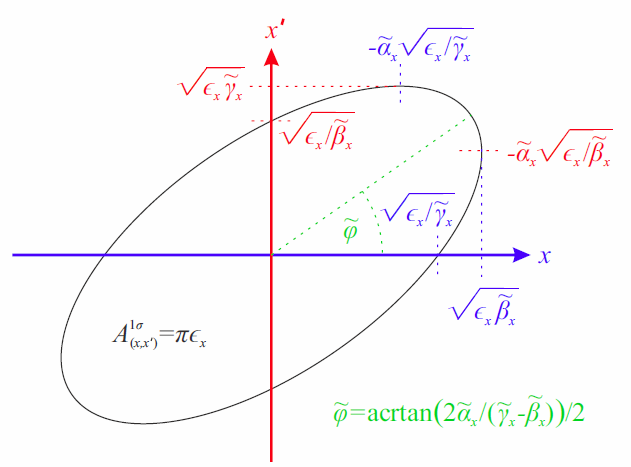
\includegraphics[scale=0.8]{phasenraum_ellipse.png}

\begin{align*}
\left(
\begin{matrix}
\beta & -\alpha \\
-\alpha & \gamma
\end{matrix}
\right)_2
=
R
\cdot 
\left(
\begin{matrix}
\beta & -\alpha \\
-\alpha & \gamma
\end{matrix}
\right)_1
\cdot 
R^T
\end{align*}
 
~ \newpage ~

$R_{56}-$Definition:

\url{https://www3.aps.anl.gov/forums/elegant/viewtopic.php?f=17&t=987}

\url{https://www3.aps.anl.gov/forums/elegant/viewtopic.php?f=17&t=966&p=4024&hilit=r56#p4024}

\url{}

Es gilt in linearer Näherung erster Ordnung in elegant:

\begin{align*}
\sigma_{56}=\langle s\delta\rangle &=\left\langle\left(R_{55}s_0+R_{56}\delta_0\right)\cdot\left(R_{66}\delta_0+R{65}s_0\right)\right\rangle\\
~ &=\left\langle R_{55}R_{66}s_0\delta_0+R_{56}R_{66}\delta^2_0+R_{55}R_{65}s_0^2+R_{56}R_{65}s_0\delta_0\right\rangle\\
~ &\overset{\text{no acc.}}{=}\left\langle s_0\delta_0+R_{56}\delta_0^2\right\rangle\\
~ &=\underbrace{\left\langle s_0\delta_0\right\rangle}_{{\sigma_{56}}_0}  +   R_{56}\left\langle \delta_0^2\right\rangle
\end{align*}

Index 0 ist der Startpunkt. Falls am Ursprung ($s=0$), folgt:

\begin{align*}
\sigma_{56} &= \langle s\delta\rangle = R_{56}\left\langle \delta_0^2\right\rangle\\
\Leftrightarrow R_{56}  &= \frac{\sigma_{56}}{\left\langle \delta_0^2\right\rangle}=\frac{\langle s\delta\rangle}{\left\langle \delta_0^2\right\rangle}
\end{align*}

R56 = ds/ddelta, where delta=(p-p0)/p0, p0 being the initial momentum (i.e., prior to acceleration).


Wenn nicht beschleunigt wird, gilt ferner $\delta=\delta_0$. If there is no acceleration, R55=R66=1 and R65=0. A cavity with phase=0 has a non-zero R65 element, which can interact with the R56 in the chicane. You'll also see R55 change.

 

\url{https://www3.aps.anl.gov/forums/elegant/viewtopic.php?f=12&t=581&p=2336&hilit=r56#p2336}

\begin{align*}
\eta_x =etax = \sigma_{16}/\sqrt{\sigma_{66}} 
\end{align*}
wobei etax abhängig von der \glqq lokalen\grqq~energy deviation, not the energy deviation at the start of the beamline. $R_{16}$ in contrast is a transport matrix coefficient from the beginning of the beamline. etax and $R_{16}$ are different when you have acceleration.

Offene Frage: wann wird der bezug resettet? wenn energie sich ändert?


\url{https://www3.aps.anl.gov/forums/elegant/viewtopic.php?f=17&t=818&p=3379&hilit=r56#p3379}

The default for twiss\_output is to compute the local dispersion. This can be changed by setting the local\_dispersion parameter to 0. Because local\_dispersion=1 in twiss\_output, you'll see apparent inconsistencies with the transport matrix elements, which are always referenced the the initial coordinates. The local dispersion should be consistent with the effective dispersion computed from the beam moments, unless there is strong nonlinearity (e.g., if x and delta have a strong nonlinear correlation).

\url{https://www3.aps.anl.gov/forums/elegant/viewtopic.php?f=11&t=804&p=3333&hilit=r56#p3333}

In elegant, R56 is defined as ds/dpIntial, where pInitial is the momentum at the start of the beamline. In many cases, people compute ds/dpChicaneInput, which is a different number when there is acceleration. Sorry, that should be R56 = ds/dpIntial*pInitial0, etc.

\begin{align*}
\Rightarrow&~\\
~& R_{56,\text{elegant,lokal}} = \frac{ds}{\frac{dp_\text{Intial}}{p_\text{Intial,0}}} = \frac{ds}{\frac{dp_\text{Intial}}{p_\text{Final,0}}} \cdot\frac{p_\text{Intial,0}}{p_\text{Final,0}}\\
\Rightarrow&~\\
~& R_{56,\text{elegant,Start2End}} = R_{56,\text{xbeam,Sektion}_1}+R_{56,\text{xbeam,Sektion}_2}\cdot{\color{red}\frac{p_\text{Intial,0}}{p_\text{Final,0}}}\\
\Rightarrow&~\\
~& R_{56,\text{elegant,(I1)2(S)}} = R_{56,\text{xbeam,I1}}+R_{56,\text{xbeam,F}}\cdot{\color{red}\frac{p_\text{I1,0}}{p_\text{F,0}}}+R_{56,\text{xbeam,S}}\cdot{\color{red}\frac{p_\text{I1,0}}{p_\text{S,0}}}\\
\Rightarrow&~\\
~& R_{56,\text{elegant,(I0)2(S)}} = R_{56,\text{xbeam,I1}}\cdot{\color{red}\frac{p_\text{I0,0}}{p_\text{I1,0}}}+R_{56,\text{xbeam,F}}\cdot{\color{red}\frac{p_\text{I0,0}}{p_\text{F,0}}}+R_{56,\text{xbeam,S}}\cdot{\color{red}\frac{p_\text{I0,0}}{p_\text{S,0}}}
\end{align*}



\url{https://www3.aps.anl.gov/forums/elegant/viewtopic.php?f=9&t=343&p=1432&hilit=r56#p1432}

$R_{76}=d\delta/dt$

\url{https://www3.aps.anl.gov/forums/elegant/viewtopic.php?f=12&t=577&p=2312&hilit=r56#p2312}


You might try using the analyze\_map command, which also determines the matrix from traking.


 





%%%%%%%%%%%%%%%%%%%%%%%%%%%%%%%%%%%%%%%%%%%%%%%%%%%%%%%%%%%%%%%%%%%%%%%%%%%%%%%%%%%%
%%%%%%%%%%%%%%%%%%%%%%%%%%%%%%%%%%%%%%%%%%%%%%%%%%%%%%%%%%%%%%%%%%%%%%%%%%%%%%%%%%%%
%%%%%%%%%%%%%%%%%%%%%%%%%%%%%%%%%%%%%%%%%%%%%%%%%%%%%%%%%%%%%%%%%%%%%%%%%%%%%%%%%%%%


%\begin{deff}
%Definition 
%\end{deff}
%
%
%\begin{satz}
%Satz
%\end{satz}
%
%
%\begin{beweis}
%Beweis  \qed
%\end{beweis}
%
%
%\begin{theorem}
%Theorem
%\end{theorem}
%
%
%\begin{lemma}
%Lemma
%\end{lemma}
%
%
%\begin{proposition}
%Proposition
%\end{proposition}
%
%
%\begin{korollar}
%Korollar
%\end{korollar}
%
%
%\begin{bsp}
%Beispiel
%\end{bsp}
%
%
%\begin{bem}
%Bemerkung
%\end{bem}
%
%
%\begin{anm}
%Anmerkung
%\end{anm}
%
%
%\begin{folg}
%Folgerung
%\end{folg}
%
%
%\begin{wdh}
%Wiederholung
%\end{wdh}
\end{document}
